\documentclass[a4paper]{scrartcl}
%\documentclass[a4paper, 10pt]{scrartcl}
\usepackage[czech]{babel}
\usepackage[utf8]{inputenc}
\usepackage{a4wide}
\usepackage{graphicx}

\title{Děti s mimořádným nadáním}
\subtitle{Děti se specifickými potřebami}
\author{Iveta Terezie Pelikánová}
\date{}

\begin{document}

\maketitle 

\noindent

Pro tuto esej na téma "Děti se specifickými potřebami" jsem si vybrala děti s mimořádným nadáním. Toto téma mi je poměrně blízké ačkoliv jsem se s mimořádně nadanými dětmi asi nesetkala, tak se často setkávám s nadanými dospělými. Při svém studiu na ČVUT jsem potkala velké množství chytrých lidí a k mému udivení i dost lidí, o kterých jsem později zjistila, že jsou nadprůměrně inteligentní a jsou členy Mensy. Bohužel musím konstatovat, že většině z nich vysokoškolský systém učení nevyhovoval a mnoho z nich studia nedokončila. \\

V angličtině se pro vzdělávání nadaných dětí používá termín "gifted education". Dnešní školní třídy jsou plné dětí s různými diagnozami. Dyslexie, dysgrafie, ADHD, Aspergerův sydrom, poruchy autistického spektra nebo hyperaktivita a další specifické poruchy. Současně také děti s mimořádným nadáním mají specifické potřeby. Problémem diagnostiky nadaných dětí také zůstává častý souběh nadání s jiným handicapem, který maskuje rozpoznání nadání dítěte.\\

Obecně uznávanou definicí nadaných dětí je americká definice z roku 1972: "... jsou to děti, které jsou identifikovány profesionálně kvalifikovanými osobami jako děti s přednostmi význačnými pro schopnost vysokého výkonu. Tyto děti vyžadují diferencované vzdělávací programy a služby nad rámec běžně poskytovaných klasickým vzdělávacím programem k tomu, aby mohly přispět ke svému prospěchu i užitku společnosti. Děti schopné vysokého výkonu zahrnují ty, které demonstrují prospěch anebo potenciál v jakékoliv jedné či více z těchto oblastí:"\cite{def_nadane_deti}

\begin{itemize}
    \item všeobecné intelektové schopnosti
    \item specifická/jednotlivá akademická způsobilost
    \item kreativní a produktivní myšlení
    \item schopnosti vůdcovství
    \item výtvarné umění
    \item psychomotorické schopnosti
\end{itemize}

Z definice je patrné, že nadání může být velmi různé tak jako jeho projevy. V této oblasti byly vypracovány tři nejčastěji používané modely nadání: Renzulliho třífaktorový model, Mönksův vícefaktorový model a Gagného diferenciovaný model talentu a nadání. Renzulliho model spojuje tři oblasti (three-rings), jak je vidět na obrázku \ref{fig:renzulli_model}.\cite{nadani_wikipedie}

         \begin{figure}
            \centering
            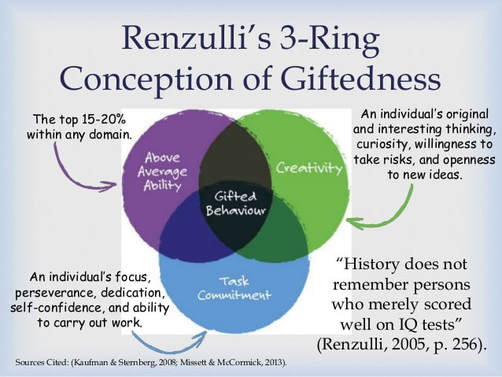
\includegraphics[width=0.8\textwidth]{renzulli_model.jpg}
            \caption{Renzulliho třífaktorový model nadání.\cite{renzuli_ring_fig}}
            \label{fig:renzulli_model}
        \end{figure}

Jde o kombinaci nadprůměrné schopnosti získávat informace (above average ability), motivace zaměřené na řešení problému (task commitment) a tvořivosti (creativity).\cite{nadani_wikipedie} Renzulli také rozlišuje dvě varianty nadání "schoolhouse giftedness" a "creative-productive giftedness", kde první ze zmíněných popisuje klasičtější představu nadání dětí, které ve škole excelují, jsou dobrými počtáři, rychle čtou a dokážou dobře procházet školním prostředím, a druhá skupina jsou děti velmi kreativní, které naopak ve standardizovaných testech a školním prostředí jsou těžko rozpoznatelné, protože mohou mít s klasickým školním prostředím problémy.\cite{renzuli_ring_fig}\\

Mönksův model vychází z Rezolliniho třífaktorového modelu a rozšiřuje ho o působení třech sociálních faktorů rodiny, přátel a školy, jak ukazuje obrázek \ref{fig:monks_model}.\\

        \begin{figure}
            \centering
            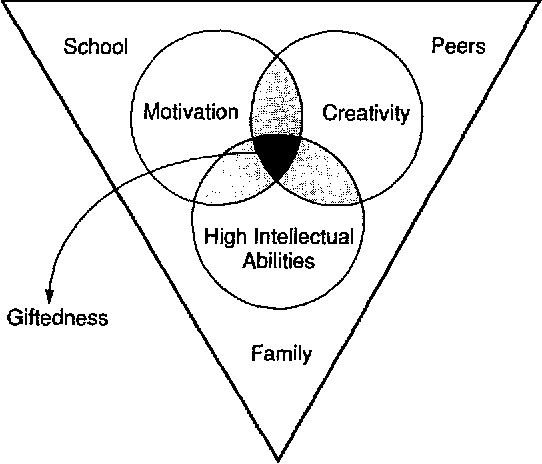
\includegraphics[width=0.6\textwidth]{monks_model.png}
            \caption{Mönksův vícefaktorový model nadání.\cite{monks_model_fig}}
            \label{fig:monks_model}
        \end{figure}

Poslední zmiňovaný diferencovaný model nadání dle kanadského psychologa Francoyse Gagného rozlišuje přirozené schopnosti a schopnosti rozvíjené, jak ukazuje obrázek \ref{fig:gagne_model}. Přirozené schopnosti, které popisují nadání, dělí do pěti kategorií - intelektové, kreativní, sociální a senzomotorické. Tyto přirozené schopnosti se vyvíjí působením prostředí, náhod a katalyzátorů v systematicky rozvíjených schopnostech, které Gagné kategorizuje do schopností akademických, umění, obchodních, zálib, sociálních aktivit, sportů a technologií.\cite{gagne_model_fig}\\

        \begin{figure}
            \centering
            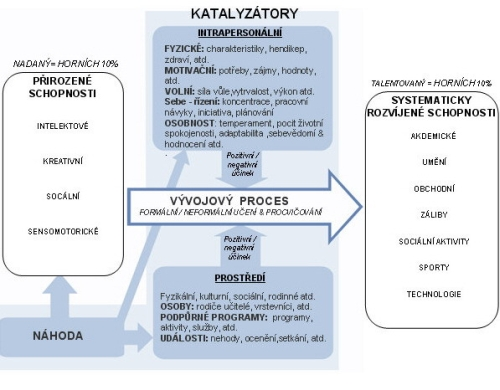
\includegraphics[width=\textwidth]{gagne_model.jpg}
            \caption{Gagného diferencovaný model nadání.\cite{gagne_model_fig}}
            \label{fig:gagne_model}
        \end{figure}

Jaké jsou tedy nejtypičtější projevy nadaných dětí? Vysoká inteligence, bohatá slovní zásoba, bystrá mysl, vysoká vnímavost, brzy čtou, mají více různých zájmů, spojování zdánlivě nesmyslných věcí do smysluplných souvislostí, rády tráví čas se staršími dětmi či dospělými, často si nerozumí s vrstevníky, dokáží se koncentrovat po dlouho dobu, jsou samostatnější a rychleji se učí než děti stejného věku.\cite{nadani_wikipedie,tak_mali} Tyto projevy patří do tzv. pozitivních projevů. Nadané děti se ale mohou projevovat také negativně. Mohou odmítat práci či pracovat nedbale, jsou nervózní při tempu práce třídy, protestují proti rutinní a předvídatelné práci, sní v průběhu dne, bývají panovančí k učitelům i spolužákům, odmítají se podřídit, "hrají divadlo" a ruší spolužáky, nebo se mohou stát "třídními šašky".\cite{def_nadane_deti} Nadané děti jsou ale každé jedinečné. Jak jsem již zmiňovala velkou skupinu tvoří děti tzv. twice exceptional s dvojí vyjímečností. Nejčastějšími kombinacemi handikapu a nadání jsou nadané děti se specifickými vývojovými poruchami učení, zejména s dyslexií, dysortografií, dysgrafií, nadané děti s poruchami chování ADHD, ADD a nadané děti s Aspergerovým syndromem. Tyto handikapy mohou značně ztížit rozlišení nadání kvůli stereotypním očekávání, že děti s určitou poruchou jsou mentálně podprůměrné.\cite{dvoji_vyjimecnost}\\

V tomto ohledu je velmi důležitá pečlivá diagnostika poruch chování a učení u dětí. Mezi nejstarší možnosti diagnostiky nadaných dětí je měření jejich inteligence (IQ). Tato měření a testy mají největší tradici (přes 100 let), ale bohužel nepostihují celou šíři škály nadání. Odborníci doporučují širší strategii identifikace nadaných dětí, aby nešlo pouze o jednorázovou činnost. Renzulli a Reis navrhují čtyři etapy identifikace:
    
    \begin{itemize}
        \item navržení na základě výsledku testu - standardizované inteligenční a výkonostní testy
        \item navržení učitelem - konzultace s učitelem, který žáka dobře zná (nejlépe s třídním učitelem)
        \item alternativní cesty - nominace dalšími lidmi, které dítě znají, rodiče, vrstevníci, lidé, které dítě navrhne, a výsledky testu tvořivosti
        \item závěrečný návrh / bezpečnostní krok - návrhy ostatních učitelů, aby byla korigována osobní sympatie jednoho učitele k žákovi \cite{def_nadane_deti}
    \end{itemize}
    
O tuto problematiku je v české i světové pedagogice v současnosti poměrně zájem. Českému prostředí se snaží nadané děti přiblížit například pedagožka Monika Stehlíková svými publikacemi Život s vysokou inteligencí - průvodce pro nadané dospělé a nadané děti \cite{} a Nadané dítě - jak mu pomoci ke štěstí a úspěchu \cite{}



\vspace{36pt}
\indent Tento text byl vypracován k udělení zápočtu z předmětu {\it Specifické poruchy učení a chování}.

\newpage
\bibliographystyle{unsrt} % We choose the "plain" reference style
\bibliography{reference} % Entries are in the "refs.bib" file

\end{document}